\documentclass[UTF8,openany,zihao=-4,scheme=chinese]{ctexbook}

\usepackage[a4paper,margin=2.5cm]{geometry}
\usepackage{amsmath,amssymb}
\usepackage{booktabs,longtable,array}
\usepackage{enumitem}
\usepackage{xcolor}
\usepackage{listings}
\usepackage{tikz}
\usepackage{url}
\usepackage{hyperref}
\usetikzlibrary{arrows.meta,positioning,shapes.multipart,fit,calc}

\hypersetup{
  colorlinks=true,
  linkcolor=blue!55!black,
  citecolor=blue!55!black,
  urlcolor=blue!55!black,
  pdftitle={AFEPack 中文使用说明},
  pdfauthor={AFEPack project}
}

\definecolor{codebg}{RGB}{248,248,248}
\definecolor{codeframe}{RGB}{210,210,210}
\definecolor{commentgreen}{RGB}{54,120,54}
\definecolor{keywordblue}{RGB}{30,70,150}

\lstdefinestyle{afecode}{
  backgroundcolor=\color{codebg},
  frame=single,
  rulecolor=\color{codeframe},
  basicstyle=\ttfamily\small,
  keywordstyle=\color{keywordblue}\bfseries,
  commentstyle=\color{commentgreen},
  stringstyle=\color{purple!60!black},
  showstringspaces=false,
  breaklines=true,
  columns=fullflexible,
  keepspaces=true,
  tabsize=2,
  numbers=left,
  numberstyle=\scriptsize\color{gray},
  xleftmargin=1.5em,
  framexleftmargin=1.2em
}
\lstset{style=afecode}

\newcommand{\file}[1]{\nolinkurl{#1}}
\newcommand{\class}[1]{\texttt{#1}}
\newcommand{\cmd}[1]{\texttt{#1}}

\tikzset{
  umlclass/.style={
    draw,
    rectangle split,
    rectangle split parts=3,
    rectangle split part align={center,left,left},
    text width=5.1cm,
    align=left,
    rounded corners=1pt,
    fill=white,
    font=\scriptsize,
    inner sep=4pt
  },
  umlsmall/.style={
    draw,
    rectangle split,
    rectangle split parts=3,
    rectangle split part align={center,left,left},
    text width=4.15cm,
    align=left,
    rounded corners=1pt,
    fill=white,
    font=\scriptsize,
    inner sep=3pt
  },
  layer/.style={
    draw,
    rounded corners=2pt,
    minimum height=1.0cm,
    text width=12.5cm,
    align=center,
    font=\small\bfseries
  },
  flow/.style={
    draw,
    rounded corners=2pt,
    align=center,
    text width=4.0cm,
    minimum height=1.05cm,
    fill=white,
    font=\scriptsize,
    inner sep=4pt
  },
  assoc/.style={-{Stealth[length=2.5mm]},thick},
  dep/.style={-{Stealth[length=2.5mm]},thick,dashed},
  inherit/.style={-{Triangle[length=3mm,width=3mm]},thick}
}

\title{AFEPack 中文使用说明}
\author{根据当前项目文档、源码与示例整理}
\date{\today}

\begin{document}

\frontmatter
\maketitle
\tableofcontents

\chapter{前言}

AFEPack 是一个面向有限元与自适应有限元程序开发的 C++ 类库。当前源码树同时保留了早期 Texinfo 手册、中文安装说明、头文件接口和五个示例程序\cite{afepack-source}。本文档根据这些本地材料整理，重点解释当前仓库中的实际使用方式，而不是逐字翻译旧手册。

本文使用 \class{ctexbook} 文档类编写，参考文献由 BibTeX 管理，类关系和流程图由 TikZ 绘制。主要依据包括：

\begin{itemize}[leftmargin=2em]
  \item \file{INSTALL_CN.md}：当前 Autotools 构建、依赖检查、MPI 与 gmsh 测试选项；
  \item \file{doc/AFEPack.texi}：AFEPack 的设计目标、三层架构、模板单元和自适应网格说明；
  \item \file{include/AFEPack/*.h}：当前可用类、函数和命名空间接口；
  \item \file{examples/*}：Poisson、变系数椭圆方程、2D 局部加密和 3D 示例；
  \item \file{tools/README}：网格和可视化格式转换工具。
\end{itemize}

\section*{读者对象}

本文假定读者已经熟悉弱形式、有限元空间、单元矩阵、数值积分和 Dirichlet 边界条件。若需要系统学习有限元理论，可参考 Ciarlet 的有限元专著和 Brenner--Scott 教材\cite{ciarlet1978fem,brenner2008mathematical}。

\mainmatter

\chapter{总体结构}

\section{设计目标}

AFEPack 的核心目标是把有限元程序中的三类变化点显式拆开：

\begin{enumerate}[leftmargin=2em]
  \item 网格几何：由 \class{Mesh<DIM,DOW>}、\class{EasyMesh}、\class{GmshMesh} 和层次网格类管理；
  \item 模板单元：由模板几何、自由度分布、坐标变换和基函数共同定义；
  \item 离散算子：由 \class{BilinearOperator} 及其派生类装配为稀疏矩阵。
\end{enumerate}

这种拆分使用户可以在同一套全局自由度管理和装配框架下替换单元类型、基函数、网格来源和双线性型。旧手册称 AFEPack 由有限元模块、自适应网格模块和应用模块三层组成\cite{afepack-texinfo}；当前源码仍然基本保持这个分层。

\begin{figure}[htbp]
\centering
\begin{tikzpicture}[node distance=0.45cm]
  \node[layer,fill=blue!8] (app) {应用层：用户方程、误差估计、时间推进、示例程序};
  \node[layer,fill=green!8,below=of app] (op) {离散与求解层：\class{BilinearOperator}、\class{Operator}、\class{BoundaryConditionAdmin}、\class{AMGSolver}};
  \node[layer,fill=yellow!12,below=of op] (fem) {有限元空间层：\class{TemplateElement}、\class{FEMSpace}、\class{Element}、\class{FEMFunction}};
  \node[layer,fill=orange!12,below=of fem] (mesh) {网格与模板数据层：\class{Mesh}、\class{EasyMesh}、\class{GmshMesh}、\class{HGeometryTree}、模板文件};
  \node[layer,fill=gray!12,below=of mesh] (la) {基础设施：\class{Vector}、\class{SparseMatrix}、\class{SparsityPattern}、CBLAS/LAPACKE、Boost.Serialization};
  \draw[assoc] (la) -- (mesh);
  \draw[assoc] (mesh) -- (fem);
  \draw[assoc] (fem) -- (op);
  \draw[assoc] (op) -- (app);
\end{tikzpicture}
\caption{AFEPack 当前源码树中的主要层次}
\label{fig:layers}
\end{figure}

\section{核心类关系}

图 \ref{fig:fem-uml} 是单网格有限元程序最常见的类关系。实际接口都在 \file{include/AFEPack} 中声明；图中只列出用户最常接触的成员。

\begin{figure}[htbp]
\centering
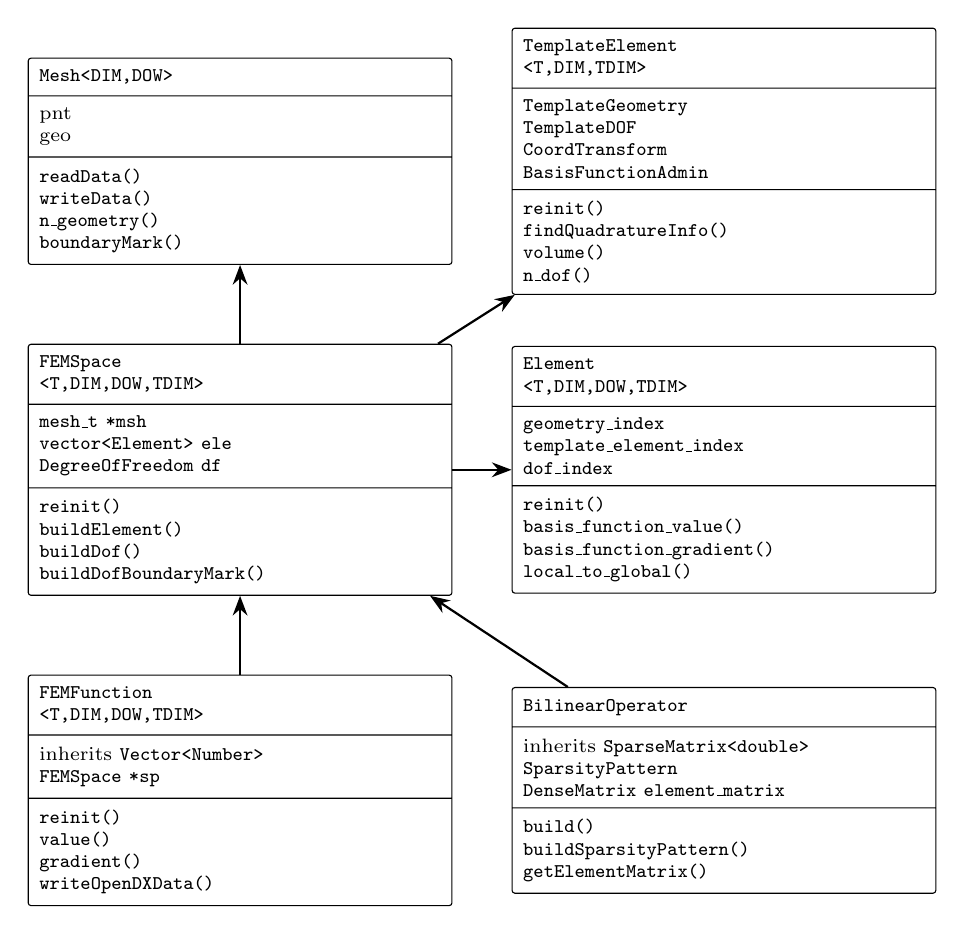
\begin{tikzpicture}[node distance=1.0cm and 0.75cm]
  \node[umlclass] (mesh) {
    \class{Mesh<DIM,DOW>}
    \nodepart{second}
    \file{pnt}\\
    \file{geo}
    \nodepart{third}
    \class{readData()}\\
    \class{writeData()}\\
    \class{n\_geometry()}\\
    \class{boundaryMark()}
  };
  \node[umlclass,right=of mesh] (tmpl) {
    \class{TemplateElement}\\
    \class{<T,DIM,TDIM>}
    \nodepart{second}
    \class{TemplateGeometry}\\
    \class{TemplateDOF}\\
    \class{CoordTransform}\\
    \class{BasisFunctionAdmin}
    \nodepart{third}
    \class{reinit()}\\
    \class{findQuadratureInfo()}\\
    \class{volume()}\\
    \class{n\_dof()}
  };
  \node[umlclass,below=of mesh] (space) {
    \class{FEMSpace}\\
    \class{<T,DIM,DOW,TDIM>}
    \nodepart{second}
    \class{mesh\_t *msh}\\
    \class{vector<Element> ele}\\
    \class{DegreeOfFreedom df}
    \nodepart{third}
    \class{reinit()}\\
    \class{buildElement()}\\
    \class{buildDof()}\\
    \class{buildDofBoundaryMark()}
  };
  \node[umlclass,right=of space] (ele) {
    \class{Element}\\
    \class{<T,DIM,DOW,TDIM>}
    \nodepart{second}
    \class{geometry\_index}\\
    \class{template\_element\_index}\\
    \class{dof\_index}
    \nodepart{third}
    \class{reinit()}\\
    \class{basis\_function\_value()}\\
    \class{basis\_function\_gradient()}\\
    \class{local\_to\_global()}
  };
  \node[umlclass,below=of space] (fun) {
    \class{FEMFunction}\\
    \class{<T,DIM,DOW,TDIM>}
    \nodepart{second}
    inherits \class{Vector<Number>}\\
    \class{FEMSpace *sp}
    \nodepart{third}
    \class{reinit()}\\
    \class{value()}\\
    \class{gradient()}\\
    \class{writeOpenDXData()}
  };
  \node[umlclass,right=of fun] (bilin) {
    \class{BilinearOperator}
    \nodepart{second}
    inherits \class{SparseMatrix<double>}\\
    \class{SparsityPattern}\\
    \class{DenseMatrix element\_matrix}
    \nodepart{third}
    \class{build()}\\
    \class{buildSparsityPattern()}\\
    \class{getElementMatrix()}
  };
  \draw[assoc] (space) -- (mesh);
  \draw[assoc] (space) -- (tmpl);
  \draw[assoc] (space) -- (ele);
  \draw[assoc] (fun) -- (space);
  \draw[assoc] (bilin) -- (space);
\end{tikzpicture}
\caption{单网格有限元程序中的核心类关系}
\label{fig:fem-uml}
\end{figure}

\section{典型求解流程}

一个稳态椭圆问题的程序通常遵循图 \ref{fig:workflow}。示例 \file{examples/poisson_equation/poisson_equation.cpp} 和 \file{examples/poisson_equation_3D/poisson_equation.cpp} 都采用这个结构。

\begin{figure}[htbp]
\centering
\begin{tikzpicture}[node distance=0.8cm and 0.55cm]
  \node[flow] (mesh) {读入网格\\\class{EasyMesh}\\\class{readData}\\或 \class{Mesh::readData}};
  \node[flow,right=of mesh] (template) {读模板单元\\\class{TemplateGeometry}\\\class{TemplateDOF}\\\class{BasisFunctionAdmin}};
  \node[flow,right=of template] (space) {建立空间\\\class{FEMSpace}\\\class{buildElement}\\\class{buildDof}};
  \node[flow,below=of space] (matrix) {装配矩阵\\\class{StiffMatrix}\\\class{build}\\或派生矩阵};
  \node[flow,left=of matrix] (rhs) {离散右端\\\class{Operator}\\\class{L2Discretize}};
  \node[flow,left=of rhs] (bc) {施加边界\\\class{BoundaryConditionAdmin}\\\class{apply}};
  \node[flow,below=of bc] (solve) {求解线性系统\\\class{AMGSolver}\\\class{solve}};
  \node[flow,right=of solve] (post) {后处理\\\class{writeOpenDXData}\\\class{Functional::L2Error}};
  \draw[assoc] (mesh) -- (template);
  \draw[assoc] (template) -- (space);
  \draw[assoc] (space) -- (matrix);
  \draw[assoc] (matrix) -- (rhs);
  \draw[assoc] (rhs) -- (bc);
  \draw[assoc] (bc) -- (solve);
  \draw[assoc] (solve) -- (post);
\end{tikzpicture}
\caption{AFEPack 求解椭圆型方程的常用流程}
\label{fig:workflow}
\end{figure}

\chapter{安装与运行环境}

\section{依赖}

当前源码树的构建系统基于 Autotools。与旧 Texinfo 手册不同，当前版本不再把 deal.II 作为构建依赖；基础线性代数由项目自带类配合 CBLAS/LAPACKE 完成。Debian/Ubuntu 上的串行构建依赖为：

\begin{lstlisting}[language=bash]
sudo apt update
sudo apt install build-essential libopenblas-dev liblapacke-dev \
                 libboost-serialization-dev
\end{lstlisting}

若要重新生成 \file{configure} 和 \file{Makefile.in}，还需要：

\begin{lstlisting}[language=bash]
sudo apt install autoconf automake libtool
\end{lstlisting}

3D 示例测试依赖 gmsh\cite{gmsh2009}；启用 MPI 构建时需要 OpenMPI 或兼容 MPI C++ 编译器：

\begin{lstlisting}[language=bash]
sudo apt install gmsh
sudo apt install libopenmpi-dev openmpi-bin
\end{lstlisting}

\section{串行构建}

推荐使用源码树外构建目录：

\begin{lstlisting}[language=bash]
mkdir -p build
cd build
CC=gcc CXX=g++ ../configure
make -j"$(nproc)"
make test
make install
\end{lstlisting}

默认安装前缀为 \file{$HOME/local/AFEPack}。如需指定位置：

\begin{lstlisting}[language=bash]
CC=gcc CXX=g++ ../configure --prefix="$HOME/local/AFEPack"
\end{lstlisting}

当前 \file{configure.ac} 会检查 C++20、\file{cblas.h}、\file{lapacke.h} 和 Boost.Serialization。若系统 OpenBLAS 同时提供 CBLAS 与 LAPACKE，可使用 \cmd{--with-openblas-libdir=DIR}；若二者来自不同目录，应分别使用 \cmd{--with-cblas-libdir} 和 \cmd{--with-lapacke-libdir}。

\section{可选功能}

\begin{longtable}{>{\ttfamily}p{0.36\textwidth}p{0.56\textwidth}}
\toprule
选项 & 说明\\
\midrule
\endfirsthead
\toprule
选项 & 说明\\
\midrule
\endhead
--enable-debug & 使用调试编译选项。\\
--enable-mpi & 构建 MPI 相关库并安装 MPI 头文件，默认关闭。\\
--enable-gmsh-tests=auto|yes|no & 控制 3D/gmsh 示例测试，默认 \cmd{auto}。\\
--with-cblas-includedir=DIR & 指定 CBLAS 头文件目录。\\
--with-cblas-libdir=DIR & 指定 CBLAS 库目录。\\
--with-lapacke-includedir=DIR & 指定 LAPACKE 头文件目录。\\
--with-lapacke-libdir=DIR & 指定 LAPACKE 库目录。\\
--with-boost=DIR & 指定 Boost 安装前缀。\\
--with-boost-libdir=DIR & 指定 Boost 库目录。\\
\bottomrule
\end{longtable}

\section{运行环境变量}

安装后的示例和用户程序通常需要：

\begin{lstlisting}[language=bash]
export LD_LIBRARY_PATH="$HOME/local/AFEPack/lib:${LD_LIBRARY_PATH}"
export AFEPACK_PATH="$HOME/local/AFEPack/include/AFEPack"
export AFEPACK_TEMPLATE_PATH="$AFEPACK_PATH/template/triangle"
\end{lstlisting}

3D 四面体示例应把模板目录切换到：

\begin{lstlisting}[language=bash]
export AFEPACK_TEMPLATE_PATH="$AFEPACK_PATH/template/tetrahedron"
\end{lstlisting}

\file{examples/*/run.sh.sample.in} 展示了安装后运行示例的最小环境设置。

\chapter{网格、模板单元与数据文件}

\section{网格类}

\class{Mesh<DIM,DOW>} 是内部网格格式的核心类，其中 \class{DIM} 表示单元拓扑维数，\class{DOW} 表示嵌入空间维数。它维护点数组和不同维数几何体数组，主要接口包括 \class{readData()}、\class{writeData()}、\class{n\_point()}、\class{n\_geometry()} 和 \class{boundaryMark()}。

常用派生或转换类如下：

\begin{longtable}{p{0.28\textwidth}p{0.64\textwidth}}
\toprule
类或工具 & 用途\\
\midrule
\endfirsthead
\toprule
类或工具 & 用途\\
\midrule
\endhead
\class{EasyMesh} & 读写 easymesh 的 2D \file{.n/.s/.e} 文件，并可输出 OpenDX 网格数据。\\
\class{GmshMesh} & 读取 gmsh 3D 数据；当前源码注释说明主要用于纯四面体网格，并可附加边界标号。\\
\class{SimplestMesh} & 只含点和单元顶点连接关系的简化网格，可生成 AFEPack 内部 \class{Mesh}。\\
\file{tools/easymesh2mesh} & easymesh 到内部 mesh 格式转换。\\
\file{tools/gmsh2mesh} & gmsh 到内部 mesh 格式转换。\\
\file{tools/mesh_refine} & 内部 mesh 格式的全局加密。\\
\bottomrule
\end{longtable}

示例中的 2D 网格由 easymesh 生成：

\begin{lstlisting}[language=bash]
easymesh D
./run.sh D
\end{lstlisting}

3D 示例先由 gmsh 生成 \file{.msh}，再转换和加密：

\begin{lstlisting}[language=bash]
gmsh -3 Cube.geo
gmsh2mesh Cube.msh Cube.mesh
mesh_refine 3 Cube.mesh Cube3.mesh 3 0
./run.sh Cube3.mesh
\end{lstlisting}

\section{模板单元组成}

AFEPack 的模板单元不是一个单独文件，而是由四组信息合成：

\begin{enumerate}[leftmargin=2em]
  \item \class{TemplateGeometry<TDIM>}：参考单元几何、体积函数和数值积分公式；
  \item \class{CoordTransform<TDIM,DIM>}：参考单元与实际单元之间的坐标变换及 Jacobian；
  \item \class{TemplateDOF<TDIM>}：自由度在参考几何体上的分布；
  \item \class{BasisFunctionAdmin<value\_type,DIM,TDIM>}：基函数值与梯度函数。
\end{enumerate}

当前仓库随源码提供多种模板，例如：

\begin{itemize}[leftmargin=2em]
  \item \file{include/AFEPack/template/interval}：1D 区间模板；
  \item \file{include/AFEPack/template/triangle}：2D 三角形、DG、RT、Morley、边元等模板；
  \item \file{include/AFEPack/template/tetrahedron}：3D 四面体模板；
  \item \file{include/AFEPack/template/twin_triangle}、\file{twin_tetrahedron}、\file{four_tetrahedron}：自适应网格中使用的复合单元模板。
\end{itemize}

\section{在程序中装配模板单元}

\file{examples/poisson_equation/poisson_equation.cpp} 给出了最短路径：

\begin{lstlisting}[language=C++]
TemplateGeometry<2> triangle_template_geometry;
triangle_template_geometry.readData("triangle.tmp_geo");

CoordTransform<2,2> triangle_coord_transform;
triangle_coord_transform.readData("triangle.crd_trs");

TemplateDOF<2> triangle_template_dof(triangle_template_geometry);
triangle_template_dof.readData("triangle.1.tmp_dof");

BasisFunctionAdmin<double,2,2> triangle_basis_function(
    triangle_template_dof);
triangle_basis_function.readData("triangle.1.bas_fun");

std::vector<TemplateElement<double,2,2> > template_element(1);
template_element[0].reinit(triangle_template_geometry,
                           triangle_template_dof,
                           triangle_coord_transform,
                           triangle_basis_function);
\end{lstlisting}

这些文件名是在运行时从 \cmd{AFEPACK\_TEMPLATE\_PATH} 搜索的。若程序报找不到模板文件或动态库，应先检查该环境变量是否指向正确的模板目录。

\section{模板文件与动态库}

模板几何和基函数数据文件通常会引用动态库中的 C 函数，例如体积函数、坐标变换、基函数值和梯度函数。对应源文件位于模板目录，例如 \file{triangle.volume.c}、\file{triangle.crd_trs.c} 和 \file{triangle.1.bas_fun.c}。安装时这些源文件会编译为模板动态库，供 \class{TemplateGeometry}、\class{CoordTransform} 和 \class{BasisFunctionAdmin} 运行时加载。

自定义模板单元时，需要保持数据文件、函数名和动态库导出符号一致。若用 C++ 编译这些函数，应使用 \class{extern "C"} 避免符号名改编。

\chapter{有限元空间与函数}

\section{建立 \class{FEMSpace}}

有了网格和模板单元后，有限元空间的建立分为四步：

\begin{enumerate}[leftmargin=2em]
  \item 用网格和模板单元数组初始化 \class{FEMSpace}；
  \item 为每个几何单元创建一个 \class{Element}，并指定模板单元编号；
  \item 调用 \class{buildElement()} 建立单元内部几何映射；
  \item 调用 \class{buildDof()} 和 \class{buildDofBoundaryMark()} 建立全局自由度及边界标号。
\end{enumerate}

\begin{lstlisting}[language=C++]
FEMSpace<double,2> fem_space;
fem_space.reinit(mesh, template_element);

int n_element = mesh.n_geometry(2);
fem_space.element().resize(n_element);
for (int i = 0; i < n_element; ++i) {
  fem_space.element(i).reinit(fem_space, i, 0);
}

fem_space.buildElement();
fem_space.buildDof();
fem_space.buildDofBoundaryMark();
\end{lstlisting}

这里第三个参数 \cmd{0} 表示所有几何单元都使用 \cmd{template\_element[0]}。在自适应或混合单元程序中，可以根据 \class{GeometryBM::n\_vertex()} 或材料标号选择不同模板。

\section{\class{Element} 的作用}

\class{Element} 是实际网格单元与模板单元之间的桥。它保存几何单元编号、模板单元编号和局部自由度到全局自由度的映射，并提供：

\begin{itemize}[leftmargin=2em]
  \item \class{basis\_function\_value()} 和 \class{basis\_function\_gradient()}：在实际单元点上计算基函数值和梯度；
  \item \class{local\_to\_global()} 和 \class{global\_to\_local()}：参考单元与实际单元坐标变换；
  \item \class{local\_to\_global\_jacobian()}：数值积分中需要的 Jacobian；
  \item \class{findQuadratureInfo()}：按代数精度查找积分公式。
\end{itemize}

因此，用户重载单元矩阵时通常只操作 \class{Element}，不直接操作全局网格数组。

\section{\class{FEMFunction}}

\class{FEMFunction<value\_type,DIM,DOW,TDIM,Number>} 继承自 \class{Vector<Number>}，表示定义在某个 \class{FEMSpace} 上的有限元函数。它既能作为线性系统的未知向量，又能在单元上求值、求梯度和输出。

常用接口：

\begin{lstlisting}[language=C++]
FEMFunction<double,2> solution(fem_space);
double uh = solution.value(point, element);
std::vector<double> grad = solution.gradient(point, element);
solution.writeOpenDXData("u.dx");
\end{lstlisting}

示例程序常用 \class{Functional::L2Error} 与解析解比较：

\begin{lstlisting}[language=C++]
double error = Functional::L2Error(
    solution, FunctionFunction<double>(&u), 3);
\end{lstlisting}

\chapter{算子装配、边界条件与求解}

\section{内置矩阵类}

\class{BilinearOperator} 是装配双线性型的抽象基类，继承 \class{SparseMatrix<double>}。它管理两个有限元空间、稀疏结构、局部单元矩阵和积分精度。用户通常使用或派生以下类：

\begin{itemize}[leftmargin=2em]
  \item \class{StiffMatrix<DIM,value\_type>}：标准刚度矩阵；
  \item \class{MassMatrix<DIM,value\_type>}：质量矩阵；
  \item \class{L2InnerProduct<DIM,value\_type0,value\_type1>}：两个空间上的 $L^2$ 内积矩阵；
  \item 自定义 \class{BilinearOperator} 派生类：重载 \class{getElementMatrix()}。
\end{itemize}

最简单的刚度矩阵装配如下：

\begin{lstlisting}[language=C++]
StiffMatrix<2,double> stiff_matrix(fem_space);
stiff_matrix.algebricAccuracy() = 4;
stiff_matrix.build();
\end{lstlisting}

\section{变系数单元矩阵}

\file{examples/elliptic_equation} 展示了扩展方式：定义 \class{Matrix : public StiffMatrix<DIM,double>}，重载 \class{getElementMatrix()}，在积分点上计算系数 $a(x)$ 并累加局部矩阵。

\begin{lstlisting}[language=C++]
class Matrix : public StiffMatrix<DIM,double>
{
public:
  Matrix(FEMSpace<double,DIM>& sp) : StiffMatrix<DIM,double>(sp) {}

  void getElementMatrix(
      const Element<double,2>& ele0,
      const Element<double,2>& ele1,
      const ActiveElementPairIterator<DIM>::State state) override;
};
\end{lstlisting}

局部积分的典型模式是：

\begin{lstlisting}[language=C++]
double volume = ele0.templateElement().volume();
const QuadratureInfo<DIM>& quad =
    ele0.findQuadratureInfo(algebricAccuracy());

std::vector<double> jacobian =
    ele0.local_to_global_jacobian(quad.quadraturePoint());
std::vector<Point<DIM> > q_point =
    ele0.local_to_global(quad.quadraturePoint());

auto basis_grad = ele0.basis_function_gradient(q_point);

for (int l = 0; l < quad.n_quadraturePoint(); ++l) {
  double Jxw = quad.weight(l) * jacobian[l] * volume;
  double a_val = a(q_point[l]);
  for (int j = 0; j < n_ele_dof; ++j)
    for (int k = 0; k < n_ele_dof; ++k)
      elementMatrix(j,k) +=
          Jxw * a_val * innerProduct(basis_grad[j][l],
                                     basis_grad[k][l]);
}
\end{lstlisting}

这个结构是 AFEPack 自定义 PDE 的关键：有限元空间、稀疏结构和全局装配由框架负责，用户只需要给出单元积分。

\section{右端项与投影}

\class{Operator} 命名空间提供 $L^2$ 插值、投影和离散化。Poisson 示例中使用解析函数离散右端项：

\begin{lstlisting}[language=C++]
Vector<double> right_hand_side;
Operator::L2Discretize(&f, fem_space, right_hand_side, 4);
\end{lstlisting}

常用函数包括：

\begin{itemize}[leftmargin=2em]
  \item \class{Operator::L2Interpolate}：插值解析函数或有限元函数；
  \item \class{Operator::L2Project}：按指定方法和积分精度做 $L^2$ 投影；
  \item \class{Operator::L2Discretize}：把函数离散成右端向量。
\end{itemize}

\section{边界条件}

\class{BoundaryConditionInfo} 定义了 \class{DIRICHLET}、\class{NEUMANN} 和 \class{ROBIN} 三个类型，但当前头文件注释明确指出实际支持重点是 Dirichlet 条件。示例中按边界标号添加多个 Dirichlet 条件：

\begin{lstlisting}[language=C++]
BoundaryFunction<double,2> boundary1(
    BoundaryConditionInfo::DIRICHLET, 1, &u);
BoundaryFunction<double,2> boundary2(
    BoundaryConditionInfo::DIRICHLET, 2, &u);

BoundaryConditionAdmin<double,2> boundary_admin(fem_space);
boundary_admin.add(boundary1);
boundary_admin.add(boundary2);
boundary_admin.apply(stiff_matrix, solution, right_hand_side);
\end{lstlisting}

边界标号来自网格中的 \class{boundaryMark()}。若边界条件没有生效，通常应先检查网格生成器和转换工具是否保留了期望的边界标号。

\section{AMG 求解器}

\class{AMGSolver} 是 AFEPack 内置的代数多重网格求解器，适合求解由刚度矩阵产生的稀疏正定系统。其实现说明引用了 Brezina 等和 Cleary 等关于 AMG 投影算子的工作\cite{brezina2000amg,cleary2000robust}。

\begin{lstlisting}[language=C++]
AMGSolver solver(stiff_matrix);
solver.solve(solution, right_hand_side, 1.0e-8, 200);
\end{lstlisting}

若在时间步进或非线性迭代中反复求解相同稀疏结构的系统，可使用 lazy 模式：

\begin{lstlisting}[language=C++]
AMGSolver solver;
solver.lazyReinit(stiff_matrix);
solver.solve(solution, right_hand_side);
\end{lstlisting}

\chapter{自适应网格与多网格操作}

\section{层次几何模型}

自适应模块围绕层次几何树组织。图 \ref{fig:adaptive-uml} 总结了主要类。

\begin{figure}[htbp]
\centering
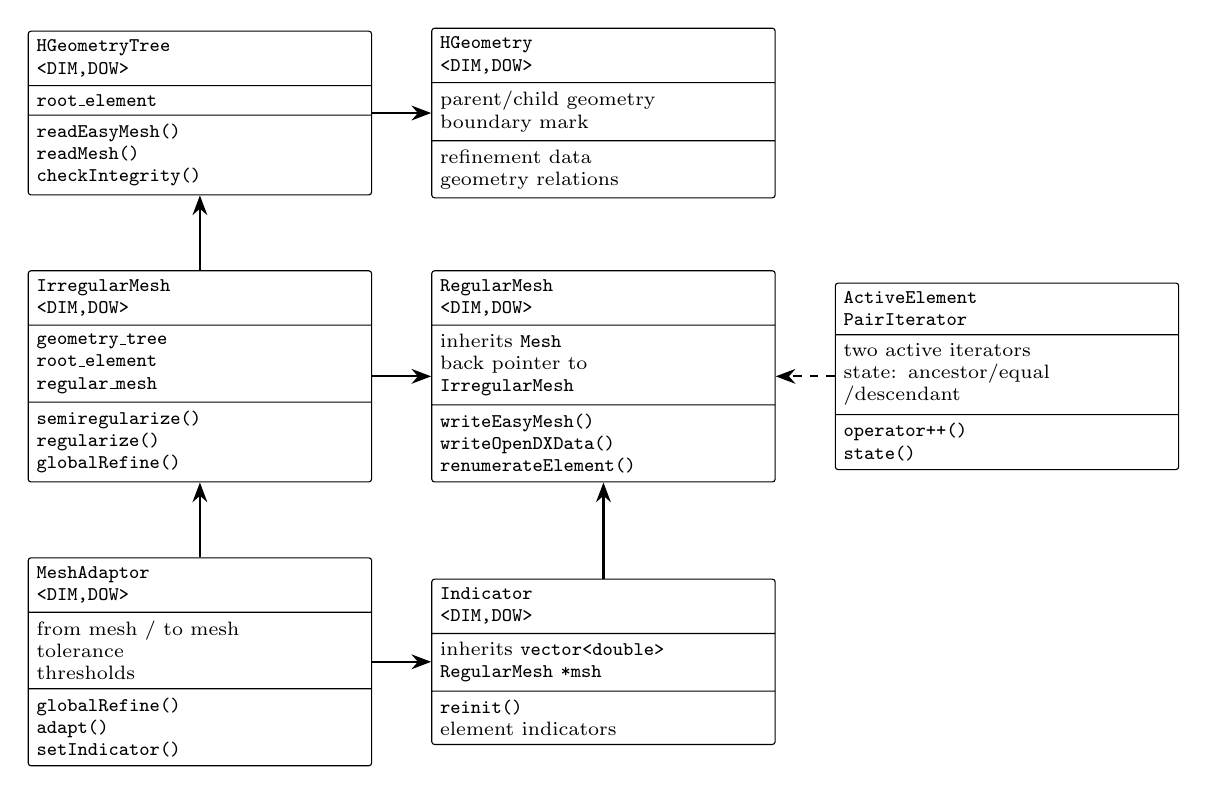
\begin{tikzpicture}[node distance=0.95cm and 0.75cm]
  \node[umlsmall] (tree) {
    \class{HGeometryTree}\\
    \class{<DIM,DOW>}
    \nodepart{second}
    \class{root\_element}
    \nodepart{third}
    \class{readEasyMesh()}\\
    \class{readMesh()}\\
    \class{checkIntegrity()}
  };
  \node[umlsmall,right=of tree] (hgeo) {
    \class{HGeometry}\\
    \class{<DIM,DOW>}
    \nodepart{second}
    parent/child geometry\\
    boundary mark
    \nodepart{third}
    refinement data\\
    geometry relations
  };
  \node[umlsmall,below=of tree] (ir) {
    \class{IrregularMesh}\\
    \class{<DIM,DOW>}
    \nodepart{second}
    \class{geometry\_tree}\\
    \class{root\_element}\\
    \class{regular\_mesh}
    \nodepart{third}
    \class{semiregularize()}\\
    \class{regularize()}\\
    \class{globalRefine()}
  };
  \node[umlsmall,right=of ir] (reg) {
    \class{RegularMesh}\\
    \class{<DIM,DOW>}
    \nodepart{second}
    inherits \class{Mesh}\\
    back pointer to\\
    \class{IrregularMesh}
    \nodepart{third}
    \class{writeEasyMesh()}\\
    \class{writeOpenDXData()}\\
    \class{renumerateElement()}
  };
  \node[umlsmall,below=of ir] (adaptor) {
    \class{MeshAdaptor}\\
    \class{<DIM,DOW>}
    \nodepart{second}
    from mesh / to mesh\\
    tolerance\\
    thresholds
    \nodepart{third}
    \class{globalRefine()}\\
    \class{adapt()}\\
    \class{setIndicator()}
  };
  \node[umlsmall,right=of adaptor] (ind) {
    \class{Indicator}\\
    \class{<DIM,DOW>}
    \nodepart{second}
    inherits \class{vector<double>}\\
    \class{RegularMesh *msh}
    \nodepart{third}
    \class{reinit()}\\
    element indicators
  };
  \node[umlsmall,right=of reg] (pair) {
    \class{ActiveElement}\\
    \class{PairIterator}
    \nodepart{second}
    two active iterators\\
    state: ancestor/equal\\
    /descendant
    \nodepart{third}
    \class{operator++()}\\
    \class{state()}
  };
  \draw[assoc] (tree) -- (hgeo);
  \draw[assoc] (ir) -- (tree);
  \draw[assoc] (ir) -- (reg);
  \draw[assoc] (ind) -- (reg);
  \draw[assoc] (adaptor) -- (ind);
  \draw[assoc] (adaptor) -- (ir);
  \draw[dep] (pair) -- (reg);
\end{tikzpicture}
\caption{自适应网格和多网格相关类}
\label{fig:adaptive-uml}
\end{figure}

\section{单网格自适应流程}

自适应网格一般遵循：

\begin{enumerate}[leftmargin=2em]
  \item 用 \class{HGeometryTree} 读入粗网格；
  \item 基于同一棵树建立 \class{IrregularMesh}；
  \item 调用 \class{semiregularize()} 和 \class{regularize()} 生成可用于 \class{FEMSpace} 的 \class{RegularMesh}；
  \item 计算每个活动单元上的误差指示子，写入 \class{Indicator}；
  \item 用 \class{MeshAdaptor} 根据指示子细化或粗化；
  \item 重新 regularize，重建有限元空间并求解。
\end{enumerate}

旧手册中的最小框架仍然可作为理解入口：

\begin{lstlisting}[language=C++]
HGeometryTree<2> tree;
tree.readEasyMesh("D");

IrregularMesh<2> irregular_mesh(tree);
irregular_mesh.semiregularize();
irregular_mesh.regularize(false);

Indicator<2> indicator(irregular_mesh.regularMesh());
// fill indicator[i] using an estimator

MeshAdaptor<2> adaptor(irregular_mesh);
adaptor.convergenceOrder() = 1.0;
adaptor.refineStep() = 1;
adaptor.setIndicator(indicator);
adaptor.tolerence() = 1.0e-8;
adaptor.adapt();
\end{lstlisting}

\section{多网格和双空间算子}

AFEPack 的一个重要特性是可以在同一层次几何树上维护多个自适应网格，并在不同网格上的有限元空间之间装配双线性算子。实现关键是：

\begin{itemize}[leftmargin=2em]
  \item 多个 \class{IrregularMesh} 必须来自同一个 \class{HGeometryTree}；
  \item \class{IrregularMeshPair} 和 \class{ActiveElementPairIterator} 遍历两个网格活动单元的交叠关系；
  \item \class{BilinearOperator} 的 \class{getElementMatrix()} 接收两个 \class{Element} 和一个 state，用于处理祖先、后代或相同单元关系；
  \item \class{L2InnerProduct}、\class{Operator::L2Project} 等接口可用于不同空间间的投影和内积。
\end{itemize}

这类程序比单网格 Poisson 示例复杂，建议把应用封装成类：成员中保存层次树、多个不规则网格、多个 \class{FEMSpace}、解函数、模板单元和误差指示子；主循环中依次执行建空间、求解、估计误差和改网格。

\chapter{示例程序导读}

\section{示例目录}

\begin{longtable}{p{0.31\textwidth}p{0.57\textwidth}}
\toprule
目录 & 说明\\
\midrule
\endfirsthead
\toprule
目录 & 说明\\
\midrule
\endhead
\file{examples/poisson_equation} & 2D Poisson 方程，easymesh 网格，输出 \file{u.dx}，计算 $L^2$ 误差。\\
\file{examples/elliptic_equation} & 2D 变系数椭圆方程，把程序封装为 \class{EllipticEquation}，并继承 \class{StiffMatrix} 自定义单元矩阵。\\
\file{examples/TaiChiYinYang} & 2D 局部加密生成太极图案，输出 \file{D.dx}。\\
\file{examples/poisson_equation_3D} & 3D Poisson 方程，gmsh 生成立方体四面体网格，输出 \file{u.dx}。\\
\file{examples/DysonSphere} & 3D 局部加密示例，使用 gmsh 网格，输出 \file{Cube.dx}。\\
\bottomrule
\end{longtable}

\section{2D Poisson 示例}

该示例求解
\[
  -\Delta u = f,\qquad
  u = \sin(\pi x)\sin(2\pi y)
\]
对应右端项为 $f=5\pi^2u$。关键代码顺序是：

\begin{enumerate}[leftmargin=2em]
  \item \class{EasyMesh mesh; mesh.readData(argv[1]);}
  \item 读取 \file{triangle.tmp_geo}、\file{triangle.crd_trs}、\file{triangle.1.tmp_dof}、\file{triangle.1.bas_fun}；
  \item 建立 \class{FEMSpace<double,2>}；
  \item 用 \class{StiffMatrix<2,double>} 装配 Laplace 刚度矩阵；
  \item 用 \class{Operator::L2Discretize} 计算右端；
  \item 对边界标号 1 到 4 添加 Dirichlet 条件；
  \item 用 \class{AMGSolver} 求解；
  \item 输出 \file{u.dx} 并打印 $L^2$ 误差。
\end{enumerate}

\section{变系数椭圆方程示例}

\file{examples/elliptic_equation} 更接近实际应用的组织方式。它把网格、模板单元、有限元空间和解函数封装为 \class{EllipticEquation} 类，并将变系数矩阵封装为 \class{Matrix}。

该示例的经验是：当问题从教学示例变成真实程序时，应把“初始化模板单元”“建立空间”“装配求解”拆成成员函数。这样后续加入网格移动、自适应或时间循环时，不需要把所有逻辑堆在 \class{main()} 中。

\section{3D Poisson 示例}

3D 示例与 2D 示例结构几乎相同，差异在于：

\begin{itemize}[leftmargin=2em]
  \item 使用 \class{Mesh<3>} 读内部 mesh 文件；
  \item 模板文件改为 \file{tetrahedron.tmp_geo}、\file{tetrahedron.crd_trs}、\file{tetrahedron.1.tmp_dof}、\file{tetrahedron.1.bas_fun}；
  \item \class{StiffMatrix<DIM,double>} 中 \cmd{DIM=3}；
  \item 运行前通常需要 \file{gmsh2mesh} 和 \file{mesh_refine} 预处理。
\end{itemize}

\chapter{常用 API 速查}

\section{网格与模板}

\begin{longtable}{p{0.36\textwidth}p{0.54\textwidth}}
\toprule
接口 & 用途\\
\midrule
\endfirsthead
\toprule
接口 & 用途\\
\midrule
\endhead
\class{Mesh<DIM,DOW>::readData(file)} & 读取 AFEPack 内部网格格式。\\
\class{Mesh<DIM,DOW>::writeData(file)} & 写出内部网格格式。\\
\class{EasyMesh::readData(prefix)} & 读取 \file{prefix.n/.s/.e}。\\
\class{TemplateGeometry::readData(file)} & 读取参考单元几何与积分信息。\\
\class{CoordTransform::readData(file)} & 读取坐标变换函数信息。\\
\class{TemplateDOF::readData(file)} & 读取模板自由度分布。\\
\class{BasisFunctionAdmin::readData(file)} & 读取基函数动态库与函数名。\\
\class{TemplateElement::reinit(...)} & 组合模板几何、自由度、坐标变换和基函数。\\
\bottomrule
\end{longtable}

\section{有限元空间与函数}

\begin{longtable}{p{0.38\textwidth}p{0.52\textwidth}}
\toprule
接口 & 用途\\
\midrule
\endfirsthead
\toprule
接口 & 用途\\
\midrule
\endhead
\class{FEMSpace::reinit(mesh, templates)} & 绑定网格和模板单元数组。\\
\class{FEMSpace::element().resize(n)} & 设置有限元空间中的单元数量。\\
\class{Element::reinit(space,i,t)} & 第 \cmd{i} 个几何单元使用第 \cmd{t} 个模板。\\
\class{FEMSpace::buildElement()} & 建立单元几何映像。\\
\class{FEMSpace::buildDof()} & 建立全局自由度编号。\\
\class{FEMSpace::buildDofBoundaryMark()} & 从几何边界标号推导自由度边界标号。\\
\class{FEMFunction::value(p,ele)} & 在单元 \cmd{ele} 内求函数值。\\
\class{FEMFunction::gradient(p,ele)} & 在单元 \cmd{ele} 内求梯度。\\
\class{FEMFunction::writeOpenDXData(file)} & 输出 OpenDX 数据。\\
\bottomrule
\end{longtable}

\section{装配与求解}

\begin{longtable}{p{0.39\textwidth}p{0.51\textwidth}}
\toprule
接口 & 用途\\
\midrule
\endfirsthead
\toprule
接口 & 用途\\
\midrule
\endhead
\class{StiffMatrix::build()} & 装配标准刚度矩阵。\\
\class{MassMatrix::build()} & 装配质量矩阵。\\
\class{BilinearOperator::algebricAccuracy()} & 设置数值积分代数精度。\\
\class{Operator::L2Discretize()} & 离散右端项。\\
\class{Operator::L2Project()} & 做 $L^2$ 投影。\\
\class{BoundaryConditionAdmin::add()} & 添加边界条件。\\
\class{BoundaryConditionAdmin::apply()} & 修改矩阵和右端以施加边界条件。\\
\class{AMGSolver::solve()} & 求解稀疏线性系统。\\
\class{Functional::L2Error()} & 计算与解析函数的 $L^2$ 误差。\\
\bottomrule
\end{longtable}

\chapter{故障诊断}

\section{构建阶段}

\begin{itemize}[leftmargin=2em]
  \item 缺少 C++20：安装较新的 \cmd{g++} 或 \cmd{clang++}，并通过 \cmd{CXX=/path/to/g++} 指定。
  \item 找不到 \file{cblas.h} 或 \file{lapacke.h}：安装 \cmd{libopenblas-dev} 与 \cmd{liblapacke-dev}，或使用 \cmd{--with-cblas-includedir}、\cmd{--with-lapacke-includedir}。
  \item CBLAS/LAPACKE 链接失败：确认头文件和库来自匹配安装；若 OpenBLAS 不含 LAPACKE 符号，不要使用组合模式 \cmd{--with-openblas-libdir}。
  \item Boost.Serialization 链接失败：安装 \cmd{libboost-serialization-dev}，或同时指定 \cmd{--with-boost} 和 \cmd{--with-boost-libdir}。
  \item 3D 测试跳过：默认 \cmd{--enable-gmsh-tests=auto} 下缺少 gmsh 会跳过，不代表库构建失败。
\end{itemize}

\section{运行阶段}

\begin{itemize}[leftmargin=2em]
  \item 找不到 \file{triangle.tmp_geo} 或 \file{tetrahedron.tmp_geo}：检查 \cmd{AFEPACK\_TEMPLATE\_PATH}。
  \item 找不到模板动态库：检查 \cmd{LD\_LIBRARY\_PATH} 是否包含 AFEPack 安装库目录，并确认模板库已安装。
  \item 边界条件不生效：检查网格文件中的边界标号，尤其是 gmsh 到内部 mesh 转换后标号是否符合程序中使用的编号。
  \item AMG 不收敛：先确认矩阵是否符合正定问题假设；再检查边界条件是否充分施加、右端项量纲和系数是否正确。
  \item OpenDX 输出不可读：确认输出文件是按节点数据还是按单元数据写出；\class{writeOpenDXData(file, flag)} 的 \cmd{flag=0} 表示位置相关数据，\cmd{flag=1} 表示连接相关数据。
\end{itemize}

\chapter{扩展建议}

\section{实现新的方程}

对一个新的二阶椭圆方程，建议按如下步骤开发：

\begin{enumerate}[leftmargin=2em]
  \item 先复用 Poisson 示例，确认网格、模板路径、边界标号和输出流程正确；
  \item 若只是常系数 Laplace，可直接使用 \class{StiffMatrix}；
  \item 若有变系数、反应项或耦合项，继承 \class{StiffMatrix}、\class{MassMatrix} 或 \class{BilinearOperator}，重载 \class{getElementMatrix()}；
  \item 用 \class{Operator::L2Discretize} 构造右端项；
  \item 用 \class{Functional} 计算误差或范数，便于回归测试。
\end{enumerate}

\section{实现新的单元}

新增单元的工作量主要在模板文件和动态库函数，而不是 \class{FEMSpace}：

\begin{itemize}[leftmargin=2em]
  \item 写参考单元几何文件和体积函数；
  \item 写坐标变换及 Jacobian；
  \item 写自由度分布文件；
  \item 写每个基函数的值和梯度函数；
  \item 在一个最小程序中读取模板并调用 \class{TemplateElement::reinit()}；
  \item 再把该模板放入 \class{FEMSpace}，用简单问题验证收敛阶。
\end{itemize}

\section{组织较大的应用}

从 \file{examples/elliptic_equation} 可以看出，较大应用不宜把所有代码写在 \class{main()} 中。推荐组织为：

\begin{itemize}[leftmargin=2em]
  \item 一个应用类保存网格、模板、有限元空间、解函数和求解参数；
  \item \class{initialize()} 只负责读网格和模板；
  \item \class{buildSpace()} 只负责重建有限元空间；
  \item \class{solve()} 只负责装配线性系统、边界条件和求解；
  \item \class{estimate()} 与 \class{adapt()} 分离，便于替换误差估计器。
\end{itemize}

\backmatter

\bibliographystyle{plain}
\bibliography{references}

\end{document}
